\section{椭圆的推导}

\begin{definition}[第一定义]
    \textbf{椭圆}是平面内一动点 $P$ 与两定点 $F_1, F_2$ 距离之和为常数 (大于 $|F_1F_2|$) 的轨迹。
\end{definition}

\begin{theorem}[椭圆方程的推导过程]
    根据椭圆定义，现有两点 $(c, 0)$,$(-c, 0)$ ，平面上有一点 A ， A 到这两点的距离之和为$2a$，其中 $a>c$ 。求 $A$ 点的轨迹。

    根据题意，得到下面方程：
    $$
        \sqrt{(x-c)^2+y^2}+\sqrt{(x+c)^2+y^2}=2 a \text{(1)}
    $$

    两侧同时乘以 $\sqrt{(x+c)^2+y^2}-\sqrt{(x-c)^2+y^2}$ ，得到下面这个方程：
    $$
        \begin{aligned}
            \frac{2 c x}{a}=\sqrt{(x+c)^2+y^2}-\sqrt{(x-c)^2+y^2} \text { (2) }
        \end{aligned}
    $$

    使用（1）+（2）可得：
    $$
        2 a+\frac{2 c x}{a}=2 \sqrt{(x+c)^2+y^2}
    $$

    两侧平方，得：
    $$
        a^2+2 c x+\frac{x^2 c^2}{a^2}=(x+c)^2+y^2
    $$

    记 $b^2=a^2-c^2$ ，移项后得到：
    $$
        \frac{x^2}{a^2}+\frac{y^2}{b^2}=1(a>b>0)
    $$
\end{theorem}

\begin{definition}[椭圆的焦点]
    椭圆的焦点是指椭圆上任意一点到两个焦点的距离之和为常数的点。设椭圆的方程为 $\frac{x^2}{a^2}+\frac{y^2}{b^2}=1(a>b>0)$，则焦点坐标为 $(\pm c, 0)$，其中 $c=\sqrt{a^2-b^2}$.
\end{definition}

\begin{theorem}[椭圆的图像]
    \begin{figure}[H]
        \centering
        \begin{minipage}[c]{0.48\textwidth}
            \centering
            \begin{tikzpicture}[scale=0.6]
                \draw[->, thick] (-4,0) -- (4,0) node[below left] {$x$};
                \draw[->, thick] (0,-3) -- (0,3) node[below left] {$y$};

                \def\a{3}
                \def\b{2}

                \draw[blue, thick] (0,0) ellipse (\a cm and \b cm);

                \pgfmathsetmacro{\c}{sqrt(\a*\a - \b*\b)}

                \coordinate (F1) at (-\c,0);
                \coordinate (F2) at (\c,0);
                \fill[red] (F1) circle (2pt) node[below] {$F_1$};
                \fill[red] (F2) circle (2pt) node[below] {$F_2$};

                \node at (0,3.5) {焦点在 $x$ 轴上的椭圆 ($\frac{x^2}{a^2} + \frac{y^2}{b^2} = 1, a>b>0$)};
            \end{tikzpicture}
        \end{minipage}
        \hfill
        \begin{minipage}[c]{0.48\textwidth}
            \centering
            \begin{tikzpicture}[scale=0.6]
                \draw[->, thick] (-3,0) -- (3,0) node[below left] {$x$};
                \draw[->, thick] (0,-4) -- (0,4) node[below left] {$y$};

                \def\a{2}
                \def\b{3}

                \draw[blue, thick] (0,0) ellipse (\a cm and \b cm);

                \pgfmathsetmacro{\c}{sqrt(\b*\b - \a*\a)}

                \coordinate (F1) at (0,-\c);
                \coordinate (F2) at (0,\c);
                \fill[red] (F1) circle (2pt) node[left] {$F_1$};
                \fill[red] (F2) circle (2pt) node[left] {$F_2$};

                \node at (0,4.5) {焦点在 $y$ 轴上的椭圆 ($\frac{x^2}{b^2} + \frac{y^2}{a^2} = 1, a>b>0$)};
            \end{tikzpicture}
        \end{minipage}
    \end{figure}
\end{theorem}

\begin{example}
    分别写出满足下列条件的动点 $P$ 的轨迹方程：
    \begin{enumerate}
        \item 点 $P$ 到点 $F_1(-3,0)$ 、$F_2(3,0)$ 的距离之和为 10 ；
        \item 点 $P$ 到点 $F_1(0,-2)$ 、$F_2(0,2)$ 的距离之和为 12 ；
        \item 点 $P$ 到点 $F_1(-4,0)$ 、$F_2(4,0)$ 的距离之和为 8 ．
    \end{enumerate}
\end{example}

\vspace{10em}

\begin{example}
    （判断正误）方程 $\frac{x^2}{m}+\frac{y^2}{n}=1(m>0, n>0)$ 不一定表示椭圆（\quad）．
\end{example}

\v{2em}

\begin{example}
    从集合 $\{3,5,7,9,11\}$ 任取两个数作为 $a, b$ ，可以得到不同的焦点在 $x$ 轴上的椭圆方程 $\frac{x^2}{a^2}+\frac{y^2}{b^2}=1$ 的个数为 （\qquad）
    \begin{tasks}(4)
        \task 25
        \task 20
        \task 10
        \task 16
    \end{tasks}
\end{example}

\vspace{4em}

\section{椭圆的长短轴和焦距}

\begin{definition}
    \begin{enumerate}
        \item 椭圆的长轴是通过椭圆中心并且与椭圆相交的最长的线段，长度为 $2a$
        \item 短轴是通过椭圆中心并且与椭圆相交的最短的线段，长度为 $2b$.
        \item 焦距为 $|F_1F_2|=2c$，其中 $c^2=a^2-b^2$.
    \end{enumerate}
\end{definition}

\begin{example}
    椭圆 $\frac{x^2}{25-k}+\frac{y^2}{9-k}=1(k<9)$ 的焦点坐标为 （\qquad），焦距是 \underline{\qquad}.
\end{example}

\v{2em}

\begin{example}
    椭圆 $\frac{x^2}{m}+y^2=1(m>0)$ 的焦点在 $x$ 轴上，长轴长是短轴长的两倍，则 $m$ 的值为 （\qquad）
    \begin{tasks}(4)
        \task $\frac{1}{4}$
        \task $\frac{1}{2}$
        \task 2
        \task 4
    \end{tasks}
\end{example}

\v{2em}

\section{求椭圆中的参数 $a,b,c$}

\begin{theorem}[椭圆的几何性质]
    \begin{enumerate}
        \item 椭圆的焦点在 $x$ 轴上时，椭圆的标准方程为 $\frac{x^2}{a^2} + \frac{y^2}{b^2} = 1 (a>b>0)$.
        \item 椭圆的焦点在 $y$ 轴上时，椭圆的标准方程为 $\frac{y^2}{a^2} + \frac{x^2}{b^2} = 1 (a>b>0)$.
        \item 椭圆的长轴长为 $2a$，短轴长为 $2b$.
    \end{enumerate}
\end{theorem}

\begin{example}
    已知 $\triangle A B C$ 的周长为 20 ，且顶点 $B(0,-4), C(0,4)$ ，则顶点 $A$ 的轨迹方程是 （\qquad）
    \begin{tasks}(4)
        \task $\frac{x^2}{36}+\frac{y^2}{20}=1(x \neq 0)$
        \task $\frac{x^2}{20}+\frac{y^2}{36}=1(x \neq 0)$
        \task $\frac{x^2}{6}+\frac{y^2}{20}=1(x \neq 0)$
        \task $\frac{x^2}{20}+\frac{y^2}{36}=1$
    \end{tasks}
\end{example}

\vspace{6em}

\section{椭圆的离心率}

\begin{definition}
    椭圆的离心率 $e$ 是椭圆的焦点到中心的距离与长轴的一半的比值，定义为：
    $$e = \frac{c}{a} = \sqrt{1 - \frac{b^2}{a^2}} (0<e<1)$$
    \begin{warning}
        椭圆离心率的取值范围是 $0<e<1$.
    \end{warning}
\end{definition}

\begin{example}
    \begin{itemize}
        \item 求椭圆 $C: \frac{x^2}{16}+\frac{y^2}{11}=1$ 的离心率 $e$.
        \item 求椭圆 $C: \frac{y^2}{16}+\frac{x^2}{11}=1$ 的离心率 $e$.
        \item 求椭圆 $C: \frac{x^2}{25}+\frac{y^2}{9}=1$ 的离心率 $e$.
    \end{itemize}
\end{example}

\v{6em}

\begin{example}
    已知椭圆 $C: \frac{x^2}{a^2}+\frac{y^2}{b^2}=1(a>b>0)$ 的左顶点与上顶点之间的距离为焦距的 $\sqrt{2}$ 倍，则 $C$ 的离心率为 \underline{\qquad}
\end{example}

\v{4em}

\begin{example}
    已知椭圆的长半轴长等于焦距的3倍，则该椭圆的离心率为 （\qquad）
    \begin{tasks}(4)
        \task $\frac{1}{8}$
        \task $\frac{1}{6}$
        \task $\frac{1}{3}$
        \task $\frac{2}{3}$
    \end{tasks}
\end{example}

\v{4em}

\begin{example}
    已知椭圆 $C: \frac{x^2}{a^2}+\frac{y^2}{4}=1(a>0)$ 的焦距为 4 ，则离心率 $e=$ （\qquad）
    \begin{tasks}(4)
        \task $\frac{1}{3}$
        \task $\frac{1}{2}$
        \task $\frac{\sqrt{2}}{2}$
        \task $\frac{2 \sqrt{2}}{3}$
    \end{tasks}
\end{example}

\v{4em}

\begin{example}
    已知椭圆 $M: \frac{x^2}{4}+\frac{y^2}{13}=1, N: \frac{x^2}{10}+y^2=1$ ，则 （\qquad）
    \begin{tasks}(4)
        \task $M$ 与 $N$ 的离心率相等
        \task $M$ 与 $N$ 的焦距相等
        \task $M$ 与 $N$ 的长轴长相等
        \task $M$ 的短轴是 $N$ 的两倍长
    \end{tasks}
\end{example}

\v{4em}

\begin{example}
    已知椭圆 $C: \frac{x^2}{a^2}+\frac{y^2}{b^2}=1(a>b>0)$ 的左、右焦点分别为 $F_1, ~ F_2$ ，点 $P$ 在椭圆 $C$ 上，若 $\left|P F_1\right|+\left|P F_2\right|=4$ ，椭圆 $C$ 的离心率为 $\frac{1}{2}$ ，则椭圆 $C$的焦距为 （\qquad）
    \begin{tasks}(4)
        \task 1
        \task 2
        \task $\sqrt{3}$
        \task $2 \sqrt{3}$
    \end{tasks}
\end{example}

\v{4em}

\begin{example}
    已知椭圆 $C: \frac{x^2}{a^2}+\frac{y^2}{b^2}=1(a>b>0)$ 的长轴长为 8 ，且离心率为 $\frac{\sqrt{15}}{4}$ ，则 $C$ 的标准方程为 \underline{\qquad}．
\end{example}

\v{4em}

\subsection{椭圆的离心率和椭圆形状的关系}

\begin{theorem}[椭圆的形状]
    椭圆的离心率 $e$ 与椭圆的形状有如下关系：
    \begin{itemize}
        \item 当 $e$ 趋近于 0 时，椭圆接近于圆形；
        \item 当 $e$ 趋近于 1 时，椭圆变得越来越扁平。
    \end{itemize}
\end{theorem}

\begin{example}
    椭圆可看成是圆被压扁或拉伸形成的．下列椭圆中，形状更接近圆的是 （\qquad）
    \begin{tasks}(4)
        \task $\frac{x^2}{25}+\frac{y^2}{9}=1$
        \task $\frac{x^2}{25}+\frac{y^2}{16}=1$
        \task $\frac{x^2}{5}+\frac{y^2}{9}=1$
        \task $\frac{x^2}{4}+y^2=1$
    \end{tasks}
\end{example}

\v{4em}

\begin{example}
    若椭圆 $C: \frac{x^2}{m}+\frac{y^2}{9}=1(m>9)$ 比椭圆 $D: \frac{x^2}{6}+\frac{y^2}{3}=1$ 更扁，则椭圆 $C$ 的长轴长的取值范围是 \underline{\qquad}.
\end{example}

\v{6em}

\section{与焦点有关的性质}

\subsection{焦半径的长度取值范围}

\begin{theorem}
    对于椭圆上一点 $P$, $PF_1 \in [a-c, a+c]$, $PF_2 \in [a-c, a+c]$.
\end{theorem}

\begin{example}
    已知椭圆 $C$ 的两个焦点分别为 $F_1(-2,0), ~ F_2(2,0)$ ，离心率为 $\frac{1}{2}$ ，且点 $P$ 是椭圆上任意一点，则下列结论正确的是 （\qquad）
    \begin{tasks}(4)
        \task $C$ 的方程为 $\frac{x^2}{16}+\frac{y^2}{12}=1$
        \task $\left|P F_2\right|_{max} = 4+\sqrt{3}$
        \task $\left|P F_1\right|=3$ 时，$\left|P F_2\right|=5$
        \task $\frac{x^2}{4}+y^2=1$ 比 $C$ 更圆
    \end{tasks}
\end{example}

\v{8em}

\subsection{利用第一定义求方程}

\begin{example}
    已知 $P$ 是椭圆 $C: \frac{x^2}{9}+\frac{y^2}{n}=1$ 上的动点，$A(-2,0), B(2,0)$ ，且 $|P A|+|P B|=6$ ，则 $n=$ \underline{\qquad}.
\end{example}

\v{6em}

\begin{example}
    已知动点 $M(x, y)$ 满足 $\sqrt{(x+3)^2+y^2}+\sqrt{(x-3)^2+y^2}=10$ ，则动点 $M$ 的轨迹方程是 \underline{\qquad}．
\end{example}

\v{6em}

\begin{example}
    平面内，动点 $P$ 的坐标 $(x, y)$ 满足方程 $\sqrt{(x+\sqrt{3})^2+y^2}+\sqrt{(x-\sqrt{3})^2+y^2}=2 \sqrt{6}$ ，则动点 $P$ 的轨迹方程为 （\qquad）
    \begin{tasks}(4)
        \task $\frac{x^2}{24}+\frac{y^2}{21}=1$
        \task $\frac{x^2}{6}+\frac{y^2}{3}=1$
        \task $\frac{x^2}{6}-\frac{y^2}{3}=1$
        \task $\frac{x^2}{9}+\frac{y^2}{6}=1$
    \end{tasks}
\end{example}

\v{4em}

\subsection{第一定义与几何关系结合}

\begin{example}
    已知动圆 $C$ 与圆 $(x-2)^2+y^2=25$ 内切，同时与圆 $(x+2)^2+y^2=1$ 外切，则动圆 $C$ 的圆心轨迹方程为 （\qquad）
    \begin{tasks}(4)
        \task $\frac{x^2}{25}+y^2=1$
        \task $\frac{x^2}{25}+\frac{y^2}{24}=1$
        \task $\frac{x^2}{9}+y^2=1$
        \task $\frac{x^2}{9}+\frac{y^2}{5}=1$
    \end{tasks}
\end{example}

\vspace{10em}

\begin{example}
    如图：已知圆 $C:(x+1)^2+y^2=25$ 内有一点 $A(1,0), ~ Q$ 是圆 $C$ 上的任意一点，线段 $A Q$ 的垂直平分线与 $C Q$ 相交点 $M$ ，当点 $Q$ 在圆 $C$ 上运动时，点 $M$ 的轨迹方程为 \underline{\qquad}
\end{example}

\begin{figure} [H]
    \centering
    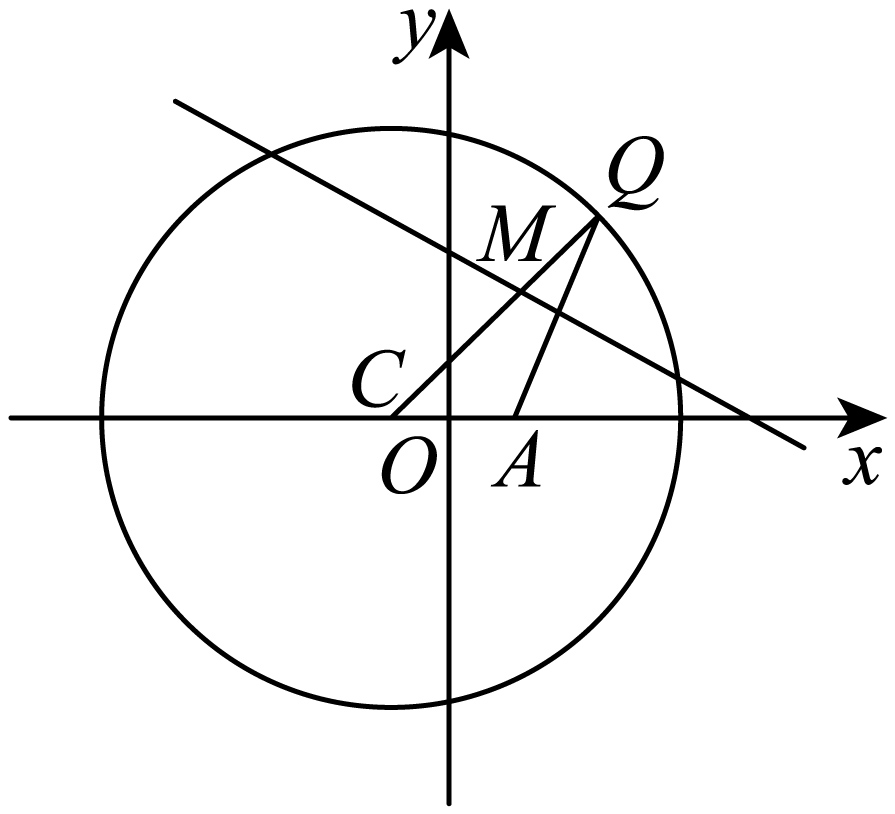
\includegraphics[width=0.25\textwidth]{chapters/圆锥曲线/images/椭圆/img-20250728135940.png}
\end{figure}

\subsection{利用第一定义求长度}

\begin{theorem}[椭圆中的 $4a$ 周长]
    过椭圆焦点的直线可能会和另一个焦点形成三角形，这个周长就是 $2a + 2a = 4a$.
\end{theorem}

\begin{example}
    椭圆 $\Gamma: \frac{x^2}{4}+\frac{y^2}{2}=1$ 的左焦点为 $F,A $、$B$ 为椭圆上两点，且直线 $A B$ 经过椭圆右焦点，则 $\triangle F A B$ 的周长为 \underline{\qquad}.
\end{example}

\v{6em}

\begin{example}
    已知椭圆 $C: \frac{y^2}{a^2}+\frac{x^2}{b^2}=1(a>b>0)$ 的上、下焦点分别为 $F_1, F_2$ ，离心率为 $\frac{2}{3}$ ，过点 $F_1$ 作直线 $l$（与 $y$ 轴不重合）交椭圆 $C$ 于 $M, N$ 两点， $\triangle M N F_2$ 的周长为 12 ，则椭圆 $C$ 的标准方程是 （\qquad）
    \begin{tasks}(4)
        \task $\frac{x^2}{3}+y^2=1$
        \task $\frac{y^2}{3}+x^2=1$
        \task $\frac{x^2}{9}+\frac{y^2}{5}=1$
        \task $\frac{y^2}{9}+\frac{x^2}{5}=1$
    \end{tasks}
\end{example}

\v{6em}

\begin{example}
    已知 $F_1, F_2$ 分别为椭圆 $C: \frac{x^2}{8}+\frac{y^2}{4}=1$ 的左、右焦点，直线 $y=2 x$ 与 $C$ 交于两点 $A, B$ ，则平行四边形 $A F_1 B F_2$ 的周长为 （\qquad）
    \begin{tasks}(4)
        \task $4 \sqrt{2}$
        \task 8
        \task $8 \sqrt{2}$
        \task 16
    \end{tasks}
\end{example}

\v{6em}

\begin{theorem}[焦点三角形的周长]
    椭圆上有一点 $P$，如果 $F_1, F_2$ 是椭圆的两个焦点，则 $\triangle F_1 P F_2$ 的周长为 $|PF_1| + |PF_2| + |F_1F_2|= 2a + 2c$
\end{theorem}

\begin{example}
    已知椭圆 $C: \frac{x^2}{12}+\frac{y^2}{16}=1$ 的两个焦点为 $F_1, ~ F_2$ ，椭圆 $C$ 上有一点 $P$ ，则 $\Delta P F_1 F_2$ 的周长为 （\qquad）
    \begin{tasks}(4)
        \task 6
        \task 16
        \task $4+4 \sqrt{3}$
        \task 12
    \end{tasks}
\end{example}

\v{6em}

\subsection{补充另一个焦点}

\begin{theorem}[常见做法：补充另一个焦点]
    如果题目只涉及到一个焦点，通常需要连接另一个焦点，产生一些微妙的关系：
    $$|PF_1|+|PF_2|=2a$$
\end{theorem}

\begin{example}
    如图，把椭圆 $\frac{x^2}{25}+\frac{y^2}{16}=1$ 的长轴 $A B$ 分成 8 等份，过每个等分点作 $x$ 轴的垂线交椭圆的上半部分于 $P_1, P_2, \cdots, P_7$ 七个点，$F$ 是椭圆的左焦点，则 $\left|P_1 F\right|+\left|P_2 F\right|+\cdots+\left|P_7 F\right|=$
    \begin{figure} [H]
        \centering
        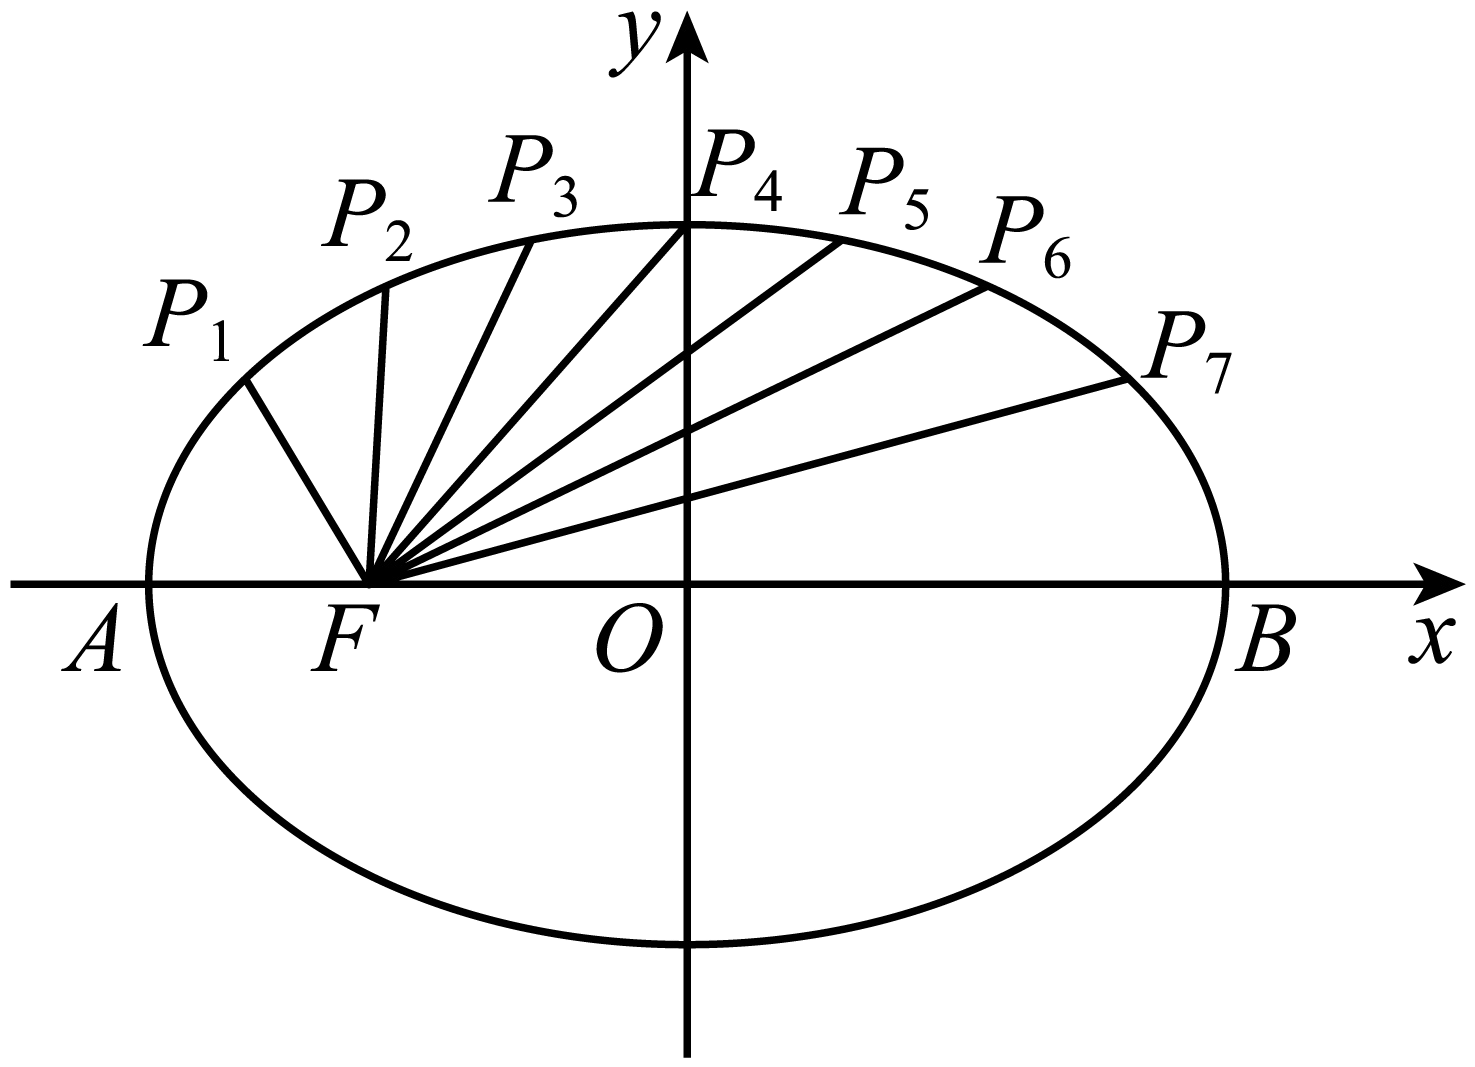
\includegraphics[width=0.25\textwidth]{chapters/圆锥曲线/images/椭圆/img-20250728135303.png}
    \end{figure}
\end{example}

\subsection{椭圆和天体运动}

\begin{theorem}[开普勒三大定律]

    \begin{enumerate}
        \item 开普勒第一定律——轨道定律：行星在不同的椭圆轨道上围绕太阳运动，太阳是在椭圆的一个焦点；
        \item 开普勒第二定律——面积定律：对每个行星来说，太阳和行星的连线在相等的时间扫过相等的面积；
        \item 开普勒第三定律——周期定律：所有行星的轨道的半长轴的三次方跟公转周期的二次方的比值都相等 即：
              $$
                  k=\frac{a^3}{T^2}
              $$
    \end{enumerate}

    \begin{corollary}[近日点和远日点]
        近日点的速度大小比远日点要大。
    \end{corollary}
\end{theorem}

\begin{example}
    如图所示，某探月卫星沿地月转移轨道飞向月球，在月球附近一点 $P$ 处变轨进入以月球球心 $F$ 为一个焦点的椭圆轨道I绕月飞行，之后卫星在 $P$点处第二次变轨进入仍以 $F$ 为一个焦点的椭圆轨道II绕月飞行，且轨道II的右顶点为轨道I的中心．设椭圆I与II的长半轴长分别为 $a_1$ 和 $a_2$ ，半焦距分别为 $c_1$ 和 $c_2$ ，离心率分别为 $e_1$ 和 $e_2$ ，则下列结论正确的是 （\qquad）
    \begin{figure} [H]
        \centering
        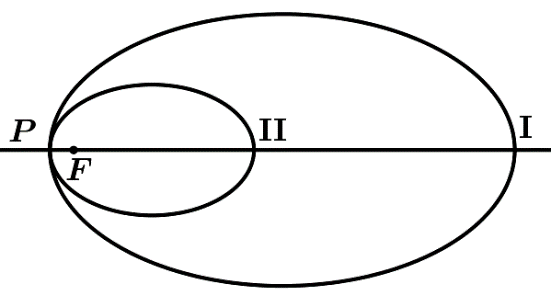
\includegraphics[width=0.25\textwidth]{chapters/圆锥曲线/images/椭圆/img-20250731012542.png}
    \end{figure}
    \begin{tasks}(4)
        \task $c_1=a_2+c_2$
        \task $a_1+c_1>2\left(a_2+c_2\right)$
        \task $e_2=2 e_1-1$
        \task 椭圆II比椭圆I更扁
    \end{tasks}
\end{example}

\v{6em}

\begin{example}
    某彗星的运行轨道是以太阳为一个焦点的椭圆．测得轨道的近日点（距离太阳最近的点）与太阳中心的距离为 $d_1$ ，远日点（距离太阳最远的点）与太阳中心的距离为 $d_2$ ，并且近日点、远日点及太阳中心在同一条直线上，则 （\qquad）
    \begin{tasks}(4)
        \task 轨道的焦距为 $d_2+d_1$
        \task 轨道的离心率为 $\frac{d_2-d_1}{d_2+d_1}$
        \task 轨道的短轴长为 $2 \sqrt{d_1 d_2}$
        \task 当 $\frac{d_1}{d_2}$ 越大时，轨道越扁
    \end{tasks}
\end{example}

\v{8em}

\begin{example}
    1970年4月24日，我国发射了自己的第一颗人造地球卫星＂东方红一号＂，从此我国开启了人造卫星的新篇章，人造地球卫星绕地球运行遵循开普勒行星运动定律：卫星在以地球为焦点的椭圆轨道上绕地球运行时，其运行速度是变化的，速度的变化服从面积守恒规律，即卫星的向径（卫星与地球的连线）在相同的时间内扫过的面积相等．设椭圆的长轴长、焦距分别为 $2 a, 2 c$ ，下列结论不正确的是 （\qquad）
    \begin{figure} [H]
        \centering
        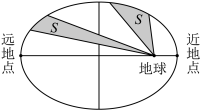
\includegraphics[width=0.22\textwidth]{chapters/圆锥曲线/images/椭圆/img-20250731013736.png}
    \end{figure}


    \begin{tasks}(4)
        \task 卫星向径的最小值为 $a-c$
        \task 卫星向径的最大值为 $a+c$
        \task* 卫星向径的最小值与最大值的比值越小，椭圆轨道越扁
        \task! 卫星运行速度在近地点时最小，在远地点时最大
    \end{tasks}
\end{example}

\v{2em}

\section{求椭圆的离心率}

\subsection{根据等式求椭圆的离心率}

\begin{theorem}
    除了最基础的定义，还要知道以下形式：
    $$ e = \sqrt{\frac{c^2}{a^2}} = \sqrt{1 - \frac{b^2}{a^2}} $$
    这个式子在警示我们，一旦知道椭圆中 $a$、$b$、$c$ 其中两个满足的等式关系，就能求出离心率，换言之，只要化简出：
    $$
        x_1a^{n_1} + x_2b^{n_2} + x_3b^{n_3} = 0
    $$
    其中，$x_1$、$x_2$、$x_3$ 这些都是常数，是可以取 $0$ 的。这个式子不需要记，只是向你展现这三个变量可以写成一个等式，那么就能求离心率。建立起了 $a$、$b$、$c$ 之间的关系，就能求出离心率的值。特别地，在等式关系里，我们可以根据定义 $e = \frac{c}{a}$，直接令 $a=1$，解出 $c$ 的值，就刚好是离心率。
\end{theorem}

\vspace{1em}

\begin{example}
    从椭圆 \(\frac{x^2}{a^2} + \frac{y^2}{b^2} = 1\)（\(a > b > 0\)），上一点 $P$ 向 $x$ 轴作垂线，垂足恰为左焦点\(F_1\)，\(A\)是椭圆与$x$轴正半轴的交点，\(B\)是椭圆与$y$轴正半轴的交点，且 \(AB\) // \(OP\) （$O$ 是坐标原点），则椭圆的离心率为 \underline{\hspace{1.5cm}}.
\end{example}

\begin{tips}
    这一道题如果把通径背下来，找到 $P$ 点的坐标的时间就能大大减少。
\end{tips}

\vspace{8em}

\begin{example}
    设椭圆 $\frac{x^2}{a^2}+\frac{y^2}{b^2}=1(a>b>0)$ 的焦距为 $2 c$ ，且 $2 b^2=3 a c$ ，则该椭圆的离心率 $e=$ \underline{\qquad}.
\end{example}

\v{8em}

\subsection{已知角度求离心率}

\begin{theorem}
    注意到离心率中 $e = \frac{c}{a}$，我们变换成 $e = \frac{2c}{2a}$，这就能把式子成和定义相关的形式：$e = \frac{|F_1F_2|}{|PF_1 PF_2|}$，使用正弦定理转换：

    在三角形中，$\angle PF_1F_2 = \alpha, \angle PF_2F_1 = \beta$，则椭圆的离心率为：
    $$e = \frac{\sin(\alpha + \beta)}{\sin \alpha + \sin \beta}$$
\end{theorem}


\begin{example}
    已知$F_1$、$F_2$是椭圆C的两个焦点，$P$是C上的一点，若$P F_1 \perp P F_2$，且$\angle P F_2 F_1 = 60^\circ$，则$C$的离心率为
    \begin{tasks}(4)
        \task $ 1- \dfrac{\sqrt{3}}{2}$
        \task $2 - \sqrt{3}$
        \task $\dfrac{\sqrt{3} - 1}{2}$
        \task $\sqrt{3} - 1$
    \end{tasks}
\end{example}

\vspace{10em}

\subsection{找几何关系求离心率}

\begin{tips}
    本质是找到 $a$、$b$、$c$ 的关系。

    一般采用余弦定理、勾股定理、相似三角形等几何关系构建等式。
\end{tips}

\begin{example}
    已知椭圆 $C: \frac{x^{2}}{a^{2}}+\frac{y^{2}}{b^{2}}=1\;(a>b>0)$ 的上顶点为 $A$ ，左、右焦点分别为 $F_{1}, F_{2}$ ，连接 $A F_{2}$并延长交椭圆 $C$ 于另一点 $B$ ，若 $|F_{1} B|:|A B|=4:5$ ，则椭圆 $C$ 的离心率为
    \begin{tasks}(4)
        \task $\frac{\sqrt{3}}{3}$
        \task $\frac{\sqrt{5}}{5}$
        \task $\frac{\sqrt{7}}{7}$
        \task $\frac{1}{3}$
    \end{tasks}
\end{example}

\vspace{10em}

\begin{example}
    已知 $F$ 为椭圆 $C: \frac{x^{2}}{a^{2}}+\frac{y^{2}}{b^{2}}=1\;(a>b>0)$ 的右焦点，$O$ 为原点， $A$ 为 $C$ 上一点， $|OA|=|OF|$ ，若 $|AF|=\frac{2a}{3}$ ，则 $C$ 的离心率为 \underline{\hspace{3cm}}.
\end{example}

\v{10em}

\begin{example}
    已知椭圆 $E: \frac{x^2}{a^2}+\frac{y^2}{b^2}=1(a>b>0)$ 的左、右焦点分别为 $F_1$、$ F_2$ ，点 $P$ 为椭圆 $E$ 上位于第一象限内的一点，若 $\left|P F_1\right|=3\left|P F_2\right|,|O P|=\left|O F_2\right|$ （ $O$ 为坐标原点），则椭圆 $E$ 的离心率为 （\qquad）
    \begin{tasks}(4)
        \task $\frac{\sqrt{5}}{4}$
        \task $\frac{\sqrt{6}}{4}$
        \task $\frac{\sqrt{2}}{2}$
        \task $\frac{\sqrt{10}}{4}$
    \end{tasks}
\end{example}

\vspace{10em}

\begin{example}
    已知椭圆 $C$ 的左右焦点分别为 $F_1 、 F_2$ ，过点 $F_2$ 的直线与椭圆 $C$ 交于点 $A, ~ B$ ，若 $\left|A F_1\right|=|A B|=5,\left|F_1 B\right|=6$ ，则椭圆 $C$ 的离心率为 \underline{\qquad} ．
\end{example}

\v{10em}

\subsection{代入点获得离心率}

\begin{theorem}
    知道一点的坐标，可以代入椭圆方程中，可以获得一个关系。

    如下题，请尝试代入点 $M$ 的坐标，得到一个关于 $a$、$b$、$c$ 的关系式。
\end{theorem}

\begin{problem}
已知 $O$ 为坐标原点，椭圆 $C: \frac{x^2}{a^2}+\frac{y^2}{b^2}=1(a>b>0)$ 的右顶点为 $A$ ，以 $O A$ 为直径的圆与椭圆 $C$ 的三个公共点分别为 $A, ~ M, ~ N$ ，若以 $O$ ，$M$ ，$A$，$N$ 为顶点的四边形是正方形，则椭圆 $C$ 的离心率为（\hspace{2em}）
\begin{tasks}(4)
    \task $\frac{2}{3}$
    \task $\frac{\sqrt{6}}{3}$
    \task $\frac{\sqrt{3}}{3}$
    \task $\frac{-1+\sqrt{5}}{2}$
\end{tasks}
\end{problem}

\v{12em}

\section{椭圆中的最值问题}

\begin{theorem}[椭圆的范围]
    在椭圆 $\frac{x^2}{a^2}+\frac{y^2}{b^2}=1(a>b>0)$ 上的点可以改写成 $x^2=a^2 (1-\frac{y^2}{b^2})$，因此 $x$ 的取值范围是 $[-a, a]$，$y$ 的取值范围是 $[-b, b]$。
\end{theorem}

\begin{example}
    已知椭圆的标准方程为 $\frac{x^2}{4}+\frac{y^2}{3}=1$ ，下列说法正确的是 （\qquad）
    \begin{tasks}(2)
        \task 椭圆的长轴长为 2
        \task 椭圆的焦点坐标为 $(\sqrt{7}, 0),(-\sqrt{7}, 0)$
        \task 椭圆关于直线 $y=x$ 对称
        \task 当点 $\left(x_0, y_0\right)$ 在椭圆上时，$\left|y_0\right| \leq \sqrt{3}$
    \end{tasks}
\end{example}

\v{4em}

\begin{example}
    已知全集 $U=\mathbf{R}$ ，集合 $M=\left\{x \left\lvert\, \frac{x^2}{4}+y^2=1\right.\right\}, N=\left\{x \left\lvert\, \frac{x-3}{x+1} \leq 0\right.\right\}$ ，则集合 $P=\{x| | 2 x+3 \mid \leq 1\}$ 可表示为 （\qquad）
    \begin{tasks}(4)
        \task $M \cap N$
        \task $M \cap \bar{N}$
        \task $M \cup N$
        \task $\bar{M} \cap N$
    \end{tasks}
\end{example}

\v{4em}

\begin{warning}
    圆锥曲线的本质是二元函数，出题人很喜欢和函数最值结合起来考察。
\end{warning}

\begin{tips}
    若问椭圆上的点到某个定点（一般是在坐标轴上，否则不好做）的距离，可以将椭圆上的这个点设为 $(x_0,y_0)$ 直接用两点间的距离公式。但代入后，会出现两个变量，此时最好的方案是利用点在椭圆上，即满足：$\frac{x_0^{2}}{a^2}+\frac{y_0^{2}}{b^2}=1$，联立两个式子消元，转化为函数最值问题。
\end{tips}

\begin{example}
    已知椭圆 $C: \frac{x^{2}}{4}+y^{2}=1$ ，则椭圆 $C$ 上的点到点 $B(0,1)$ 的距离的最大值是
    \begin{tasks}(4)
        \task $2$
        \task $\frac{16}{3}$
        \task $\frac{4 \sqrt{3}}{3}$
        \task $\sqrt{5}$
    \end{tasks}
\end{example}

\begin{tips}
    此时构造出的函数多为二次函数，注意函数由两个部分组成：解析式和定义域，缺一不可。
\end{tips}

\v{12em}

\begin{example}
    已知点 $P\left(x_0, y_0\right)$ 是椭圆 $C: \frac{x^2}{5}+y^2=1$ 上的动点，若 $A(1,0)$ ，则 $|P A|$ 的最小值为 \underline{\qquad}.
\end{example}

\v{8em}

\begin{theorem}[定一动一]
    有一个特殊情况，和圆结合起来考。这类问题常被描述为具有两个动点，求最值时，可以考虑将其中一个点定下来。求最小值，就是点到圆心的距离减去半径（$PO-r$），最大值则为（$PO+r$）。
\end{theorem}

\begin{example}
    设 $P, Q$ 分别为圆 $x^{2}+(y-6)^{2}=2$ 和椭圆 $\frac{x^{2}}{10}+y^{2}=1$ 上的点，则 $P, Q$ 两点间的最大距离是
    \begin{tasks}(4)
        \task $5 \sqrt{2}$
        \task $\sqrt{46}+\sqrt{2}$
        \task $7+\sqrt{2}$
        \task $6 \sqrt{2}$
    \end{tasks}
\end{example}

\v{12em}

\subsection{与直线距离相关的最值}

\begin{tips}
    实际上，绘制一个椭圆，再随意绘制一条不和椭圆相交的直线，大致摆弄一下，就能看出当某个点的切线和外面这条直线平行时，距离是最小的。那距离最大也比较容易考虑了。
\end{tips}

\begin{example}
    已知椭圆 $C: \frac{x^{2}}{9}+\frac{y^{2}}{4}=1$ ，则椭圆 $C$ 上的点到直线 $l: x+2 y-25=0$ 的距离的最大值为
    \begin{tasks}(4)
        \task $3 \sqrt{5}$
        \task $4 \sqrt{5}$
        \task $5 \sqrt{5}$
        \task $6 \sqrt{5}$
    \end{tasks}
\end{example}

\v{12em}

\begin{problem}
已知直线 $4x+3y-12=0$ 与 $x$ 轴、 $y$ 轴交于 $A, B$ 两点，点 $P$ 为圆 $C:(x-3)^{2}+(y-4)^{2}=4$ 上的动点，则
\begin{itemize}
    \item 直线 $AB$ 与圆 $C$ 相离
    \item $\triangle ABC$ 的面积为 $12$
    \item 当 $\angle PBA$ 最小时，$|PB|=\sqrt{5}$
    \item 点 $P$ 到直线 $AB$ 距离的最大值为 $\frac{32}{5}$
\end{itemize}
\end{problem}

\section{综合练习}

\begin{problem}
已知椭圆 $M: \frac{x^{2}}{a^{2}}+y^{2}=1\;(a>1)$ 的离心率为 $\frac{\sqrt{42}}{7}, F_{1}, F_{2}$ 是 $M$ 的焦点，$P$ 是 $M$ 上一动点， $Q$ 是圆 $N: x^{2}+(y-3)^{2}=1$ 上一动点，则
\begin{itemize}
    \item $|PF_{1}|+|PF_{2}|=2 \sqrt{7}$
    \item $M$ 的焦距为 $\sqrt{6}$
    \item $|PQ|$ 的最小值为 $1$
    \item $|PQ|$ 的最大值为 $5$
\end{itemize}
\end{problem}

\vspace{1em}

\begin{problem}
已知抛物线 $C: y^{2}=4x$ 的焦点为 $F, O$ 为坐标原点，其准线与 $x$ 轴交于点 $M$ ，经过点 $M$ 的直线 $l$ 与抛物线交于不同两点 $A(x_{1}, y_{1}), B(x_{2}, y_{2})$ ，则下列说法正确的是
\begin{itemize}
    \item $\overrightarrow{OA} \cdot \overrightarrow{OB}=5$
    \item 存在 $\angle AMF=50^{\circ}$
    \item 不存在以 $AB$ 为直径且经过焦点 $F$ 的圆
    \item 当 $\triangle ABF$ 的面积为 $4 \sqrt{2}$ 时，直线 $l$ 的倾斜角为 $\frac{\pi}{6}$ 或 $\frac{5 \pi}{6}$
\end{itemize}
\end{problem}

\section{椭圆的大题}

\subsection{与向量相关}

\begin{tips}
    最常考的是 $\overrightarrow{OA} \cdot \overrightarrow{OB}$ 的形式，设出两点坐标，可得 $x_1x_2 + y_1y_2$，再通过点 $(x_1, y_1), (x_2, y_2)$ 满足在直线上，通常可以将 $y_1$ 与 $y_2$ 转写为和 $x_1, x_2$ 有关的形式，接着再使用联立解出韦达定理即可。
\end{tips}

\vspace{1em}

\begin{theorem}
    下面介绍一个常见的向量构造：以 MN 为直径的圆。如果这个点在以 MN 为直径的圆上，那么根据圆周角为直角，可以得到两个向量点乘为零。通过简单的画图分析，显然能够清晰：

    当该点在以 MN 为直径的圆之外时，向量点乘 $> 0 (cos\theta > 0)$，在之内时，张角为钝角，那么 $cos\theta < 0 $。
\end{theorem}

\vspace{1em}

\begin{example}
    已知双曲线 $C: \frac{x^{2}}{a^{2}}-\frac{y^{2}}{b^{2}}=1\;(a>0, b>0)$ ，若 $C$ 与双曲线 $x^{2}-\frac{y^{2}}{3}=1$ 有相同的渐近线，且 $C$ 的焦点与虚轴的端点为顶点的四边形的面积为 $16 \sqrt{3}$.

    \begin{itemize}
        \item 求 $C$ 的方程；
        \item 设过 $C$ 右焦点 $F$ 的直线 $l$ 与 $C$ 交于 $A, B$ 两点，以 $AB$ 为直径圆恰好过原点，求直线 $l$ 的方程．
    \end{itemize}
\end{example}

\v{12em}

\begin{example}
    已知椭圆 $C: \frac{x^2}{a^2}+\frac{y^2}{b^2}=1(a>b>0)$ 的长轴长是短轴长的 2 倍，焦距是 $2 \sqrt{3}$ ．
    \begin{itemize}
        \item （1）求椭圆 $C$ 的方程；
        \item （2）若直线 $l: x-m y-4=0$ 与椭圆 $C$ 交于两个不同点 $D$、$E$ ，以线段 $D E$ 为直径的圆经过原点，求实数 $m$ 的值；
    \end{itemize}
\end{example}

\v{12em}

\section{椭圆 CheetSheet}

\begin{theorem}
    \begin{tabular}{| p{2cm} | >{\centering\arraybackslash}p{8cm} | >{\centering\arraybackslash}p{6cm} |}
        \hline
        \textbf{名称}         & \textbf{焦点在 $x$ 轴上}                                                                                                       & \textbf{焦点在 $y$ 轴上}                             \\
        \hline
        第一定义                & \multicolumn{2}{c|}{平面内一动点 $P$ 与两定点 $F_1, F_2$ 距离之和为常数 (大于 $|F_1F_2|$) 的轨迹}                                                                                                 \\
        \hline
        第二定义                & \multicolumn{2}{c|}{平面内一动点到定点与到准线的距离比是常数的点的轨迹 $e = \frac{MF}{d_1}$}                                                                                                         \\
        \hline
        焦点                  & \multicolumn{2}{c|}{焦点在 $x$ 轴上}                                                                                                                                             \\
        \hline
        \multirow{2}{*}{图形} & \multicolumn{2}{c|}{\underline{\quad \quad \quad \quad \quad \quad \quad \quad \quad \quad \quad \quad \quad}}                                                              \\ % Underline for x-axis ellipse graph
                            & \multicolumn{2}{c|}{\underline{\quad \quad \quad \quad \quad \quad \quad \quad \quad \quad \quad \quad \quad}}                                                              \\ % Underline for y-axis ellipse graph
        \hline
        标准方程                & $\frac{x^2}{a^2} + \frac{y^2}{b^2} = 1 (a>b>0)$                                                                           & $\frac{y^2}{a^2} + \frac{x^2}{b^2} = 1 (a>b>0)$ \\
        \hline
        范围                  & $-a \le x \le a, -b \le y \le b$                                                                                          & $-b \le x \le b, -a \le y \le a$                \\
        \hline
        顶点                  & $A_1(-a,0), A_2(a,0), B_1(0,-b), B_2(0,b)$                                                                                & $A_1(0,-a), A_2(0,a), B_1(-b,0), B_2(b,0)$      \\
        \hline
        轴长                  & \multicolumn{2}{c|}{长轴长 $=2a$, 短轴长 $=2b$, 焦距 $=|F_1F_2|=2c$, $c^2=a^2-b^2$}                                                                                                 \\
        \hline
        焦点                  & $F_1(-c,0), F_2(c,0)$                                                                                                     & $F_1(0,-c), F_2(0,c)$                           \\
        \hline
        焦半径                 & $|PF_1| = a+ex_0, |PF_2| = a-ex_0$                                                                                        & $|PF_1| = a-ey_0, |PF_2| = a+ey_0$              \\
        \hline
        离心率                 & \multicolumn{2}{c|}{$e = \frac{c}{a} = \sqrt{1 - \frac{b^2}{a^2}} (0<e<1)$}                                                                                                 \\
        \hline
        准线方程                & $x = \pm \frac{a^2}{c}$                                                                                                   & $y = \pm \frac{a^2}{c}$                         \\
        \hline
        切线方程                & $\frac{x_0x}{a^2} + \frac{y_0y}{b^2} = 1$                                                                                 & $\frac{y_0y}{a^2} + \frac{x_0x}{b^2} = 1$       \\
        \hline
        通径                  & \multicolumn{2}{c|}{过椭圆焦点且垂直于 $x$ 轴的弦长 $|AB| = \frac{2b^2}{a}$}                                                                                                             \\
        \hline
        \multirow{5}{*}{焦点三角形}
                            & \multicolumn{2}{c|}{(1) 由定义可知: $|PF_1| + |PF_2| = 2a$, 周长为: $2a + 2c$}                                                                                                      \\
        \cline{2-3}
                            & \multicolumn{2}{c|}{(2) 焦点三角形面积: $S_{\triangle PF_1F_2} = b^2 \tan \frac{\theta}{2}$}                                                                                       \\
        \cline{2-3}
                            & \multicolumn{2}{c|}{(3) 当 $P$ 在椭圆短轴上时, 夹角 $\theta$ 最大, $\cos \theta = 1-2e^2$}                                                                                              \\
        \cline{2-3}
                            & \multicolumn{2}{c|}{(4) 焦长公式: $|PF_1| = \frac{b^2}{a-c \cos \alpha}, |MF_1| = \frac{b^2}{a+c \cos \alpha}$}                                                                 \\
        \cline{2-3}
                            & \multicolumn{2}{c|}{$|MP|^2 = \frac{2ab^2}{a^2-c^2 \cos^2 \alpha} + \frac{b^2 c^2 \sin^2 \alpha}{a^2-c^2 \cos^2 \alpha}$}                                                   \\
        \cline{2-3}
                            & \multicolumn{2}{c|}{(5) 离心率: $e = \frac{\sin (\alpha+\beta)}{\sin \alpha + \sin \beta}$}                                                                                    \\
        \hline
    \end{tabular}

\end{theorem}


% % \section*{模块三 椭圆与方程} % Top-level section, not directly converted to subsubsection based on example start.

% % 内容提要
% 1．椭圆定义：设 $F_{1}, F_{2}$ 是平面上的两个定点，若平面内的点 $P$ 满足 $\left|P F_{1}\right|+\left|P F_{2}\right|=2 a$（2a＞ $\left.\left|F_{1} F_{2}\right|\right)$ ，则点 $P$ 的轨迹是以 $F_{1}, F_{2}$ 为焦点的椭圆．

% 2．椭圆的简单几何性质：

% \begin{center}
%     \begin{tabular}{|l|l|l|}
%         \hline
%         标准方程 & $\frac{x^{2}}{a^{2}}+\frac{y^{2}}{b^{2}}=1(a>b>0)$                                   & $\frac{y^{2}}{a^{2}}+\frac{x^{2}}{b^{2}}=1(a>b>0)$ \\
%         \hline
%         焦点坐标 & $F_{1}(-c, 0), \quad F_{2}(c, 0)$                                                    & $F_{1}(0, c), \quad F_{2}(0,-c)$                   \\
%         \hline
%         焦距   & \multicolumn{2}{|c|}{$\left|F_{1} F_{2}\right|=2 c$ ，且 $c^{2}=a^{2}-b^{2}$}                                                               \\
%         \hline
%         \\
%         \hline
%         范围   & $-a \leq x \leq a, \quad-b \leq y \leq b$                                            & $-b \leq x \leq b, \quad-a \leq y \leq a$          \\
%         \hline
%         对称性  & \multicolumn{2}{|c|}{关于 $x$ 轴、 $y$ 轴、原点对称}                                                                                                \\
%         \hline
%         顶点坐标 & \begin{tabular}{l}
%                    左、右顶点：$A_{1}(-a, 0), A_{2}(a, 0)$ \\
%                    上、下顶点：$B_{1}(0, b), B_{2}(0,-b)$  \\
%                \end{tabular} & \begin{tabular}{l}
%                                    左、右顶点：$B_{1}(-b, 0), \quad B_{2}(b, 0)$ \\
%                                    上、下顶点：$A_{1}(0, a), A_{2}(0,-a)$        \\
%                                \end{tabular}                                 \\
%         \hline
%         长轴长  & \multicolumn{2}{|c|}{$\left|A_{1} A_{2}\right|=2 a$ ，其中 $a$ 叫做长半轴长}                                                                       \\
%         \hline
%         短轴长  & \multicolumn{2}{|c|}{$\left|B_{1} B_{2}\right|=2 b$ ，其中 $b$ 叫做短半轴长}                                                                       \\
%         \hline
%         离心率  & \multicolumn{2}{|c|}{$e=\frac{c}{a}(0<e<1)$}                                                                                              \\
%         \hline
%     \end{tabular}
% \end{center}

% 3．通径：过椭圆焦点且垂直于长轴的弦叫做通径（如图中的两条蓝色线段），其长度为 $\frac{2 b^{2}}{a}$ ．\\

% \vspace{1em}

% \subsubsection{类型 I：椭圆定义的运用}

% \begin{example}
%     椭圆 $\frac{x^{2}}{9}+\frac{y^{2}}{2}=1$ 的焦点为 $F_{1}, F_{2}$ ，点 $P$ 在椭圆上，若 $\left|P F_{1}\right|=4$ ，则 $\left|P F_{2}\right|=$ $\qquad$ ；$\angle F_{1} P F_{2}$的大小为 $\qquad$ ；$\解三角形 P F_{1} F_{2}$ 的周长为 $\qquad$ ；若延长 $P O$ 交椭圆于 $Q$ ，则 $\left|P F_{1}\right|+\left|F_{1} Q\right|=$ $\qquad$ ．

%     解析：椭圆中给出 $\left|P F_{1}\right|$ ，可由定义求 $\left|P F_{2}\right|$ ，由题意，$a=3, b=\sqrt{2}, c=\sqrt{a^{2}-b^{2}}=\sqrt{7}$ ，\\
%     因为 $\left|P F_{1}\right|+\left|P F_{2}\right|=2 a=6$ ，且 $\left|P F_{1}\right|=4$ ，所以 $\left|P F_{2}\right|=6-\left|P F_{1}\right|=2$ ；\\
%     要求 $\angle F_{1} P F_{2}$ ，可先求 $\left|F_{1} F_{2}\right|$ ，在 $\解三角形 P F_{1} F_{2}$ 中由余弦定理推论求 $\cos \angle F_{1} P F_{2}$ ，\\
%     如图，$\left|F_{1} F_{2}\right|=2 c=2 \sqrt{7}$ ，所以 $\cos \angle F_{1} P F_{2}=\frac{\left|P F_{1}\right|^{2}+\left|P F_{2}\right|^{2}-\left|F_{1} F_{2}\right|^{2}}{2\left|P F_{1}\right| \cdot\left|P F_{2}\right|}=\frac{16+4-28}{2 \times 4 \times 2}=-\frac{1}{2}$ ，故 $\angle F_{1} P F_{2}=120^{\circ}$ ；\\
%     $\解三角形 P F_{1} F_{2}$ 的周长为 $\left|P F_{1}\right|+\left|P F_{2}\right|+\left|F_{1} F_{2}\right|=2 a+2 c=6+2 \sqrt{7}$ ；\\
%     由椭圆的对称性，$O$ 是 $P Q$ 中点，\\
%     又 $O$ 也是 $F_{1} F_{2}$ 的中点，所以四边形 $P F_{1} Q F_{2}$ 为平行四边形，\\
%     从而 $\left|Q F_{1}\right|=\left|P F_{2}\right|=2$ ，故 $\left|P F_{1}\right|+\left|Q F_{1}\right|=4+2=6$ ．\\
%     答案： $2 ; 120^{\circ} ; 6+2 \sqrt{7}$ ； 6\\
% \end{example}

% \vspace{1em}

% \begin{example}
%     （2021•新高考 I 卷）已知 $F_{1}, F_{2}$ 是椭圆 $C: \frac{x^{2}}{9}+\frac{y^{2}}{4}=1$ 的两个焦点，点 $M$ 在 $C$ 上，则 $\left|M F_{1}\right| \cdot\left|M F_{2}\right|$ 的最大值为（ ）
%     \begin{tasks}(4)
%         \task A． 13
%         \task B． 12
%         \task C． 9
%         \task D． 6
%     \end{tasks}
%     解析：由椭圆定义，$\left|M F_{1}\right|$ 与 $\left|M F_{2}\right|$ 的和为定值，故可用不等式 $m n \leq\left(\frac{m+n}{2}\right)^{2}$ 来求积的最大值，由题意，$a=3$ ，所以 $\left|M F_{1}\right|+\left|M F_{2}\right|=2 a=6$ ，故 $\left|M F_{1}\right| \cdot\left|M F_{2}\right| \leq\left(\frac{\left|M F_{1}\right|+\left|M F_{2}\right|}{2}\right)^{2}=9$ ，当且仅当 $\left|M F_{1}\right|=\left|M F_{2}\right|=3$ 时取等号，所以 $\left|M F_{1}\right| \cdot\left|M F_{2}\right|$ 的最大值为 9 ．\\
%     \textbf{答案：C}

%     【反思】涉及椭圆上的点到两焦点距离的问题，可优先往椭圆定义上思考．
% \end{example}

% \vspace{1em}

% \begin{example}
%     已知椭圆 $C: \frac{x^{2}}{4}+\frac{y^{2}}{3}=1$ 的左、右焦点分别为 $F_{1}, F_{2}, A(1,2), P$ 为植圆 $C$ 上的动点，则 $|P A|-\left|P F_{1}\right|$ 的最小值为 $\qquad$ ．

%     解析：如图，直接分析 $|P A|-\left|P F_{1}\right|$ 的最小值不易，涉及 $\left|P F_{1}\right|$ ，可考虑用椭圆定义将其转换成 $\left|P F_{2}\right|$ 来看，由题意，$\left|P F_{1}\right|+\left|P F_{2}\right|=4$ ，所以 $\left|P F_{1}\right|=4-\left|P F_{2}\right|$ ，\\
%     故 $|P A|-\left|P F_{1}\right|=|P A|-\left(4-\left|P F_{2}\right|\right)=|P A|+\left|P F_{2}\right|-4$（1），\\
%     由三角形两边之和大于第三边知 $|P A|+\left|P F_{2}\right| \geq\left|A F_{2}\right|$ ，\\
%     结合（1）得 $|P A|-\left|P F_{1}\right|=|P A|+\left|P F_{2}\right|-4 \geq\left|A F_{2}\right|-4$（2），\\
%     当且仅当点 $P$ 位于图中 $P_{0}$ 处时取等号，\\
%     椭圆的半焦距 $c=\sqrt{a^{2}-b^{2}}=\sqrt{4-3}=1$ ，所以 $F_{2}(1,0)$ ，又 $A(1,2)$ ，所以 $\left|A F_{2}\right|=2$ ，代入（2）知 $|P A|-\left|P F_{1}\right| \geq 2-4=-2$ ，故 $|P A|-\left|P F_{1}\right|$ 的最小值为 -2 ．\\
%     \textbf{答案：－2}

%     【反思】涉及椭圆上的点到一个焦点的距离的最值问题，若不易直接求解，则可考虑用椭圆定义，转化到另一个焦点去分析。
% \end{example}

% \vspace{1em}

% \subsubsection{类型 II：椭圆的标准方程与简单几何性质}

% \begin{example}
%     椭圆中心在原点，焦点在 $x$ 轴上，离心率 $e=\frac{1}{2}$ ，且过点 $(2 \sqrt{2}, \sqrt{3})$ ，则椭圆的方程为 $\qquad$ ．\\
%     解析：设椭圆的方程为 $\frac{x^{2}}{a^{2}}+\frac{y^{2}}{b^{2}}=1(a>b>0)$ ，已知离心率，可找到 $a, b, c$ 的比例关系，将变量归一化，由题意，$e=\frac{c}{a}=\frac{1}{2}$ ，所以 $a=2 c, b=\sqrt{a^{2}-c^{2}}=\sqrt{3} c$ ，故楮圆的方程为 $\frac{x^{2}}{4 c^{2}}+\frac{y^{2}}{3 c^{2}}=1$ ，最后求 $c$ ，将已知的点代入即可，椭圆过点 $(2 \sqrt{2}, \sqrt{3}) \Rightarrow \frac{8}{4 c^{2}}+\frac{3}{3 c^{2}}=1$ ，解得：$c=\sqrt{3}$ ，所以椭圆的方程为 $\frac{x^{2}}{12}+\frac{y^{2}}{9}=1$ ．\\
%     \textbf{答案：$\frac{x^{2}}{12}+\frac{y^{2}}{9}=1$}
% \end{example}

% \vspace{1em}

% \begin{example}
%     若方程 $x^{2}+k y^{2}=2$ 表示焦点在 $y$ 轴上的椭圆，则实数 $k$ 的取值范围为 $\qquad$ ．\\
%     解析：先将梢圆化为标准方程，再比较分母，$x^{2}+k y^{2}=2 \Rightarrow \frac{y^{2}}{\frac{2}{k}}+\frac{x^{2}}{2}=1$ ，\\
%     因为椭圆焦点在 $y$ 轴上，所以 $\frac{2}{k}>2$ ，解得： $0<k<1$ ．\\
%     \textbf{答案：$(0,1)$}

%     【反思】对于椭圆，若焦点在 $x$ 轴，则在其标准方程中，$x^{2}$ 的分母大；若焦点在 $y$ 轴，则 $y^{2}$ 的分母大．
% \end{example}

% \vspace{1em}

% \begin{example}
%     （2022－全国甲卷）已知椭圆 $C: \frac{x^{2}}{a^{2}}+\frac{y^{2}}{b^{2}}=1(a>b>0)$ 的离心率为 $\frac{1}{3}, A_{1}, A_{2}$ 分别为 $C$的左、右顶点，$B$ 为 $C$ 的上顶点，若 $\overrightarrow{B A_{1}} \cdot \overrightarrow{B A_{2}}=-1$ ，则 $C$ 的方程为（ ）
%     \begin{tasks}(4)
%         \task A．$\frac{x^{2}}{18}+\frac{y^{2}}{16}=1$
%         \task B．$\frac{x^{2}}{9}+\frac{y^{2}}{8}=1$
%         \task C．$\frac{x^{2}}{3}+\frac{y^{2}}{2}=1$
%         \task D．$\frac{x^{2}}{2}+y^{2}=1$
%     \end{tasks}
%     解析：已知离心率，可找到 $a, b, c$ 的比例关系，将变量归一化，\\
%     由题意，离心率 $e=\frac{c}{a}=\frac{1}{3}$ ，所以 $a=3 c, b=\sqrt{a^{2}-c^{2}}=2 \sqrt{2} c$ ，如图，$A_{1}(-3 c, 0), A_{2}(3 c, 0), B(0,2 \sqrt{2} c)$ ，所以 $\overrightarrow{B A_{1}}=(-3 c,-2 \sqrt{2} c), \overrightarrow{B A_{2}}=(3 c,-2 \sqrt{2} c)$ ，\\
%     故 $\overrightarrow{B A_{1}} \cdot \overrightarrow{B A_{2}}=-3 c \cdot 3 c+(-2 \sqrt{2} c)^{2}=-c^{2}$ ，\\
%     因为 $\overrightarrow{B A_{1}} \cdot \overrightarrow{B A_{2}}=-1$ ，所以 $-c^{2}=-1$ ，从而 $c^{2}=1$ ，\\
%     故 $a^{2}=9 c^{2}=9, b^{2}=8 c^{2}=8$ ，所以 $C$ 的方程为 $\frac{x^{2}}{9}+\frac{y^{2}}{8}=1$ ．\\
%     \textbf{答案：B}
% \end{example}

% \vspace{1em}

% \subsubsection{强化训练}

% \begin{example}
%     1. 粗圆 $\frac{y^{2}}{a^{2}}+\frac{x^{2}}{b^{2}}=1(a>b>0)$ 的右顶点为 $A(1,0)$ ，过其焦点且垂直于长轴的弦长为 1 ，则椭圆的方程为 $\qquad$ ．
% \end{example}

% \vspace{1em}

% \begin{example}
%     2. 对称轴为坐标轴的椭圆经过 $P(-2 \sqrt{3}, 1), Q(\sqrt{3},-2)$ 两点，则椭圆的方程为 $\qquad$ ．
% \end{example}

% \vspace{1em}

% \begin{example}
%     3．（2023•新高考 I 卷• $ $ ）\\
%     设椭圆 $C_{1}: \frac{x^{2}}{a^{2}}+y^{2}=1(a>1), C_{2}: \frac{x^{2}}{4}+y^{2}=1$ 的离心率分别为 $e_{1}, e_{2}$ ，若 $e_{2}=\sqrt{3} e_{1}$ ，则 $a=(\quad)$
%     \begin{tasks}(4)
%         \task A．$\frac{2 \sqrt{3}}{3}$
%         \task B．$\sqrt{2}$
%         \task C．$\sqrt{3}$
%         \task D．$\sqrt{6}$
%     \end{tasks}
% \end{example}

% \vspace{1em}

% \begin{example}
%     4．（2023•湖北武汉二调•＊＊＊）（多选）\\
%     若椭圆 $\frac{x^{2}}{m^{2}+2}+\frac{y^{2}}{m^{2}}=1(m>0)$ 的某两个顶点间的距离为 4 ，则 $m$ 的可能取值有
%     \begin{itemize}
%         \item A．$\sqrt{5}$
%         \item B．$\sqrt{7}$
%         \item C．$\sqrt{2}$
%         \item D． 2
%     \end{itemize}
% \end{example}

% \vspace{1em}

% \begin{example}
%     5．（ $\star \star \star$ ）\\
%     已知 $\解三角形 A B C$ 的周长是 8 ，且 $B(-1,0), C(1,0)$ ，则顶点 $A$ 的轨迹方程是
%     \begin{tasks}(4)
%         \task A．$\frac{x^{2}}{9}+\frac{y^{2}}{8}=1(x \neq \pm 3)$
%         \task B．$\frac{x^{2}}{9}+\frac{y^{2}}{8}=1(x \neq 0)$
%         \task C．$\frac{x^{2}}{4}+\frac{y^{2}}{3}=1(y \neq 0)$
%         \task D．$\frac{y^{2}}{4}+\frac{x^{2}}{3}=1(y \neq 0)$
%     \end{tasks}
% \end{example}

% \vspace{1em}

% \begin{example}
%     已知 $F_{1}, F_{2}$ 是椭圆 $\frac{x^{2}}{25}+\frac{y^{2}}{16}=1$ 的左、右焦点，$P$ 为椭圆上一点，$M$ 为 $F_{1} P$ 中点，$|O M|=3$ ，则 $\left|P F_{1}\right|=$ $\qquad$ ．
% \end{example}

% \vspace{1em}

% \begin{example}
%     7. 已知 $F_{1}, F_{2}$ 为椭圆 $\frac{x^{2}}{25}+\frac{y^{2}}{9}=1$ 的两个焦点，过 $F_{1}$ 的直线交椭圆于 $A, B$ 两点，若 $\left|A F_{2}\right|+\left|B F_{2}\right|=12$ ，则 $|A B|=$ $\qquad$ ．
% \end{example}

% \vspace{1em}

% \begin{example}
%     椭圆 $C: \frac{x^{2}}{4}+\frac{y^{2}}{3}=1$ 的左、右焦点分别为 $F_{1}, F_{2}, A(1,1), P$ 为椭圆 $C$ 上的动点，则 $|P A|+\left|P F_{1}\right|$ 的最大值为 $\qquad$ ．
% \end{example}